\SourcePage{739}{742}
\section{Behavior of cross sections near a reaction threshold}

If the sum of the internal energies of the reaction products exceeds that of the initial particles, the reaction has a \emph{threshold}: it can occur only when the kinetic energy $E$ of the colliding particles (in the center-of-mass system) exceeds a certain threshold value $E_{\mathrm{th}}$. We shall examine the energy dependence of the reaction cross section near this threshold. We assume that the reaction again produces only two particles (a reaction of the type $A+B=A'+B'$).

Near threshold, the relative velocity $v'$ of the particles produced is small. This reaction is inverse to one in which the velocity of the colliding particles is small. Its cross section as a function of $v'$ can therefore be obtained directly, by detailed balance (144.13), from the known energy dependence of the reaction for which $v'$ would be the velocity in the entrance channel (\S~143). For the broad class of reactions in which there is no Coulomb interaction between $A'$ and $B'$ (for example, nuclear reactions producing a slow neutron), the reaction cross section is consequently proportional to $v'^2(1/v')$, and hence\footnote{The constancy, noted at the end of \S~144, of the limit approached by the amplitude $f_{fi}$ as $p_f\to0$ is precisely consistent with this result: the cross section (144.4) is proportional to $p_f$.}
\begin{equation}
 \sigma_r\sim v'.
 \tag{147.1}
\end{equation}
\SourcePage{740}{743}
This also gives its dependence on the energy of the colliding particles: $v'$, and therefore the reaction cross section, is proportional to the square root of $E-E_{\mathrm{th}}$:
\begin{equation}
 \sigma_r=A\sqrt{E-E_{\mathrm{th}}}.
 \tag{147.2}
\end{equation}

Scattering amplitudes in the different channels are related by the unitarity conditions. Because of this relation, the opening of a new channel produces characteristic features in the energy dependence of the cross sections of other processes as well, including elastic scattering (E.~Wigner, 1948; A.~I.~Baz', 1957; G.~Breit, 1957). To establish the origin and form of this effect, consider the simplest case, in which only elastic scattering is possible below the reaction threshold.

Close to threshold, $A'$ and $B'$ are produced in a state of orbital angular momentum $l=0$ (this is exactly the condition corresponding to the law (147.2)). If the participating particles have no spin, orbital angular momentum is conserved, and the $A+B$ system is also in an $s$ state. According to (142.7), the partial reaction cross section for $l=0$ is related to the elastic-scattering element of the $S$ matrix by
\begin{equation}
 \sigma_r=\frac\pi{k^2}(1-|S_0|^2),
 \tag{147.3}
\end{equation}
where $k$ is the wave vector of the colliding particles. Equating (147.2) and (147.3), we find that above and near the threshold, to terms of order $\sqrt{E-E_{\mathrm{th}}}$, the modulus $|S_0|$ is
\begin{equation}
 |S_0|=1-\frac{k_{\mathrm{th}}^2}{2\pi}A\sqrt{E-E_{\mathrm{th}}},\qquad E>E_{\mathrm{th}},
 \tag{147.4}
\end{equation}
where $k_{\mathrm{th}}=\sqrt{2mE_{\mathrm{th}}}/\hbar$ ($m$ is the reduced mass of $A$ and $B$). Below threshold only elastic scattering occurs, so that
\begin{equation}
 |S_0|=1,\qquad E<E_{\mathrm{th}}.
 \tag{147.5}
\end{equation}

\SourcePage{741}{744}
The scattering amplitude, and hence $S_0$, must nevertheless be analytic throughout the energy domain. To the same accuracy, a function having the values (147.4) and (147.5) above and below threshold is
\begin{equation}
 S_0=e^{2i\delta_0}\left(1-\frac{k_{\mathrm{th}}^2}{2\pi}A\sqrt{E-E_{\mathrm{th}}}\right),
 \tag{147.6}
\end{equation}
where $\delta_0$ is constant. (For $E<E_{\mathrm{th}}$, the root $\sqrt{E-E_{\mathrm{th}}}$ becomes imaginary, and the modulus of the parenthesized expression differs from unity only by a higher-order small quantity.)

For every $l\ne0$, however, inelastic scattering is absent, and therefore
\begin{equation}
 S_l=e^{2i\delta_l},\qquad l\ne0,
 \tag{147.7}
\end{equation}
where, in the threshold region, each phase $\delta_l$ is to be replaced by its value at $E=E_{\mathrm{th}}$\footnote{Since the functions $\delta_l(E)$ are real both for $E>E_{\mathrm{th}}$ and for $E<E_{\mathrm{th}}$, they are expandable in integral powers of $E-E_{\mathrm{th}}$.}.

Substitution of these $S_l$ in (142.2) gives the following scattering amplitude near the reaction threshold:
\begin{equation}
 f(\theta,E)=f_{\mathrm{th}}(\theta)-\frac{k_{\mathrm{th}}}{4\pi}A
 \sqrt{E-E_{\mathrm{th}}}\,e^{2i\delta_0},
 \tag{147.8}
\end{equation}
where $f_{\mathrm{th}}(\theta)$ is the amplitude at $E=E_{\mathrm{th}}$. It follows that the differential scattering cross section is
\[
 \frac{d\sigma}{d\Omega}=
 \begin{cases}
 |f_{\mathrm{th}}(\theta)|^2+\dfrac{k_{\mathrm{th}}}{2\pi}A\sqrt{E-E_{\mathrm{th}}}
 \operatorname{Im}\{f_{\mathrm{th}}(\theta)e^{-2i\delta_0}\},&E>E_{\mathrm{th}},\\
 |f_{\mathrm{th}}(\theta)|^2-\dfrac{k_{\mathrm{th}}}{2\pi}A\sqrt{E_{\mathrm{th}}-E}
 \operatorname{Re}\{f_{\mathrm{th}}(\theta)e^{-2i\delta_0}\},&E<E_{\mathrm{th}}.
 \end{cases}
\]
Writing $f_{\mathrm{th}}=|f_{\mathrm{th}}|e^{i\alpha(\theta)}$, we obtain finally
\begin{equation}
 \frac{d\sigma}{d\Omega}=|f_{\mathrm{th}}(\theta)|^2-
 \frac{k_{\mathrm{th}}}{2\pi}A|f_{\mathrm{th}}(\theta)|\sqrt{|E-E_{\mathrm{th}}|}
 \begin{cases}
 \sin(2\delta_0-\alpha),&E>E_{\mathrm{th}},\\
 \cos(2\delta_0-\alpha),&E<E_{\mathrm{th}}.
 \end{cases}
 \tag{147.9}
\end{equation}

According as the angle $2\delta_0-\alpha$ lies in the first, second, third, or fourth quadrant, the energy dependence described by this formula has the form shown in Fig.~50a, b, c, or d. In every case there are two branches on opposite sides of a common vertical tangent.

On integrating (147.9) over $d\Omega$, only the isotropic part of $f_{\mathrm{th}}(\theta)$ contributes to the integrals of the second terms: this is the partial amplitude $(e^{2i\delta_0}-1)/(2ik_{\mathrm{th}})$ of elastic $s$-wave scattering. The total elastic-scattering cross section near threshold is therefore
\begin{equation}
 \sigma=\sigma_{\mathrm{th}}-2A\sqrt{|E-E_{\mathrm{th}}|}
 \begin{cases}
 \sin^2\delta_0,&E>E_{\mathrm{th}},\\
 \sin\delta_0\cos\delta_0,&E<E_{\mathrm{th}}.
 \end{cases}
 \tag{147.10}
\end{equation}
\SourcePage{742}{745}
This dependence has form a or b in Fig.~50, according as $\sin\delta_0\cos\delta_0$ is positive or negative.

Thus, the existence of a reaction threshold produces a characteristic feature in the energy dependence of the elastic-scattering cross section. Particle spin naturally changes the quantitative formulas, but not the general character of the phenomenon\footnote{For nonzero spins the $A'+B'$ system in an $s$ state may have nonzero total angular momentum, allowing several orbital states of the $A+B$ system.}. If reactions other than elastic scattering are also possible below threshold, analogous features occur in their cross sections. At $E=E_{\mathrm{th}}$ every such cross section has a singular point, near which it is a linear function of $\sqrt{|E-E_{\mathrm{th}}|}$, with different slopes above and below threshold.

\begin{figure}[tbp]
\centering
\begin{tikzpicture}[x=0.72cm,y=0.50cm,line cap=round,line join=round]
\foreach \yy/\lab/\m/\k/\sleft/\sright in {12/{a}/1.25/.633/-1/-1,8/{b}/.7/.4/1/-1,4/{c}/.35/.45/1/1,0/{d}/.7/.4/-1/1}{
  \draw[->] (0,\yy) -- (5.4,\yy) node[right] {$E$};
  \draw[->] (0,\yy-1.15) -- (0,\yy+1.55) node[above] {$\dfrac{d\sigma}{dE}$};
  \draw[dashed] (2.7,\yy-1.0) -- (2.7,\yy+1.35);
  \draw[smooth,samples=60,domain=.35:2.7] plot (\x,{\yy+\m+\sleft*\k*sqrt(2.7-\x)});
  \draw[smooth,samples=60,domain=2.7:5.05] plot (\x,{\yy+\m+\sright*\k*sqrt(\x-2.7)});
  \node at (2.7,\yy-1.35) {\lab};
}
\end{tikzpicture}
\caption{}
\end{figure}

In nuclear reactions that emit a positively charged particle, the reaction products $A'$ and $B'$ repel each other by Coulomb forces. In this case, as $v'\to0$ (that is, $E\to E_{\mathrm{th}}$), the reaction cross section and all its energy derivatives tend exponentially to zero; consequently, the cross sections of other processes acquire no threshold feature.

Finally, consider a reaction producing two slow particles of opposite charge, between which the Coulomb force is attractive. Detailed balance relates its cross section to the cross section (143.6) of the inverse reaction between two slow, mutually attracting particles. It follows that, as $v'\to0$, the cross section tends to a constant limit:
\begin{equation}
 \sigma_r=\mathrm{const}\quad\text{as }v'\to0,
 \tag{147.11}
\end{equation}
so that beyond threshold the reaction begins immediately with a finite cross section.

\SourcePage{743}{746}
We now determine the threshold feature of the elastic-scattering cross section in this case (A.~I.~Baz', 1959). Unlike the neutral-particle case considered above, this cannot be done directly from the known above-threshold law (147.11) by the same simple argument. The complication is that, in the near-threshold region below $E_{\mathrm{th}}$, the $A'+B'$ system has bound states corresponding to the discrete energy levels in an attractive Coulomb field. Energetically, these states can be formed in collisions of $A$ and $B$, but the possibility of elastic scattering makes them only quasistationary. Their existence must nevertheless give rise to resonance effects in subthreshold elastic scattering, analogous to Breit--Wigner resonances.

To solve the problem, consider the structure of the wave functions describing the collision. Since there are two channels, the Schrödinger equation of the interacting system has two independent solutions finite throughout configuration space; denote two arbitrarily chosen and normalized solutions by $\psi_1$ and $\psi_2$. Linear combinations of these functions can describe scattering with either channel as entrance channel. Denote by $a$ and $b$ the channels belonging to the particle pairs $A,B$ and $A',B'$, and let $\psi=a_1\psi_1+a_2\psi_2$ correspond to entrance channel $a$; it describes elastic scattering of $A$ and $B$ together with the reaction $A+B\to A'+B'$. Near threshold the coefficients $a_1,a_2$ depend essentially on the small momentum $k_b$, whereas the arbitrarily chosen functions $\psi_1,\psi_2$ themselves have no singular behavior at $k_b=0$.

At large distances, $\psi$ must be the sum of two terms describing the motion of the particle pairs in channels $a$ and $b$. Each term is the product of the particles' ``internal'' functions and the wave function for their relative motion\footnote{The law (147.11) holds not only for the total cross section but also for partial cross sections of different angular momenta $l$ (compare the end of \S~143). The threshold feature considered below therefore occurs in every partial scattering cross section. Its character is already fully revealed for $l=0$, which is the case treated below. To simplify notation, the subscript 0 is omitted from the corresponding partial amplitudes.}. In channel $a$ the latter is $R_a^- -S_{aa}R_a^+$, and in channel $b$ it is $-S_{ab}R_b^+$, where $R^+$ and $R^-$ are the outgoing and incoming waves in the corresponding channels. At distances $r_0$ large compared with the range of the short-range forces and small compared with $1/k_b$, these functions and their derivatives must match values obtained from $\psi$ in the ``reaction zone.'' The matching conditions have the form
\[
 a_1\alpha_1+a_2\alpha_2=(R_a^--S_{aa}R_a^+)|_{r_0},\qquad
 a_1\beta_1+a_2\beta_2=-S_{ab}R_b^+|_{r_0},
\]
where $\alpha_1,\alpha_2,\beta_1,\beta_2,\ldots$ are quantities calculated from $\psi_1$ and $\psi_2$; by the argument above, they may be treated near threshold as constants independent of $k_b$. Dividing corresponding members of the first and second pairs of these equations gives two linear equations for $a_1/a_2$ and $S_{aa}$. Their coefficients contain only one quantity with a ``critical'' dependence on $k_b$, namely the logarithmic derivative of the outgoing wave in channel $b$. Define it by
\[
 \Lambda=\left.\frac1{2\pi}\frac{(rR_b^+)'}{rR_b^+}\right|_{r=r_0}.
\]
There is no need to solve these equations explicitly. It is enough to observe that $S_{aa}$, which determines the elastic-scattering amplitude, is a linear-fractional function of $\Lambda$. Below threshold $\Lambda$ is real, since $R_b^+$ is real: it solves a real Schrödinger equation with the real boundary condition at infinity of decay as $e^{-\varkappa_b r}$, where $\varkappa_b=\sqrt{2m_b(E_{\mathrm{th}}-E)}/\hbar$. At the same time $|S_{aa}|=1$ below threshold. Hence the linear-fractional function $S_{aa}(\Lambda)$ must have the form
\begin{equation}
 S_{aa}=\frac{1+\beta\Lambda}{1+\beta^*\Lambda}e^{2i\eta},
 \tag{147.12}
\end{equation}
\SourcePage{744}{747}
where $\eta$ is real and $\beta$ is a complex constant.

Let us determine $\Lambda$ as a function of $k_b$. Since the force between $A'$ and $B'$ is attractive and Coulombic, $rR_b^+$ is a Coulomb wave function asymptotically proportional to $e^{ik_br}$ at infinity. In a repulsive Coulomb field this function is $G_0+iF_0$, with $G_0$ and $F_0$ given by (138.4) and (138.7). An attractive field is obtained by changing simultaneously the signs of $k$ and $r$\footnote{Coulomb units are used below. Formally, changing the signs of $k$ and $r$ corresponds to changing the sign of the Coulomb unit of length.}. Making this replacement and evaluating the logarithmic derivative (see \S~138), we obtain\footnote{For simplicity in the formulas that follow, a real constant independent of $k_b$, namely $-\ln2r_0-2C$, has been omitted from the braces. This merely amounts to an inessential redefinition of the complex quantity $\beta$ and the real quantity $\eta$ in (147.12).}
\begin{equation}
 \Lambda=\frac{i}{1-\exp(-2\pi/k_b)}-\frac1\pi
 \left\{\ln k_b+\frac12\left[\psi\left(\frac{i}{k_b}\right)+
 \psi\left(-\frac{i}{k_b}\right)\right]\right\}.
 \tag{147.13}
\end{equation}
\SourcePage{745}{748}
Here $k_b$ is assumed real, so this formula applies above threshold. As $k_b\to0$, the first term in (147.13) tends to $i$, while the second tends to zero (see the note on p.~695). Thus above threshold
\begin{equation}
 \Lambda=i,\qquad E>E_{\mathrm{th}}.
 \tag{147.14}
\end{equation}
The continuation below threshold is made by replacing $k$ with $i\varkappa$. Equation (147.13) then gives, as $\varkappa\to0$\footnote{The first term in (147.13) becomes $-(1/2)\cot(\pi/\varkappa_b)+i/2$, while the expression in braces becomes $(\pi/2)\cot(\pi/\varkappa_b)+i\pi/2$. Here one uses $\psi(x)-\psi(-x)=-\pi\cot\pi x-1/x$, obtainable by logarithmic differentiation of $\Gamma(x)\Gamma(-x)=-\pi/(x\sin\pi x)$, together with the limiting form $\psi(x)\approx\ln x-1/2x$ as $x\to\infty$.}
\begin{equation}
 \Lambda=\cot\frac\pi{\varkappa_b},\qquad E<E_{\mathrm{th}}.
 \tag{147.15}
\end{equation}

These formulas answer the question posed. The elastic-scattering cross section is
\[
 \sigma_e=\frac\pi{k_a^2}|S_{aa}-1|^2.
\]
Above threshold,
\begin{equation}
 S_{aa}=\frac{1+i\beta}{1+i\beta^*}e^{2i\eta}.
 \tag{147.16}
\end{equation}
Like the reaction cross section, the scattering cross section is constant in this region. Notice that $|S_{aa}|\leq1$ requires $\operatorname{Im}\beta>0$.

Below threshold we find
\begin{equation}
 S_{aa}=e^{2i\eta}\frac{\beta-\tan(\pi/\varkappa_b)}
 {\beta^*-\tan(\pi/\varkappa_b)}.
 \tag{147.17}
\end{equation}
\SourcePage{746}{749}
This expression has infinitely many resonances accumulating toward $E=E_{\mathrm{th}}$. The resonance energies are the roots of $S_{aa}=-1$, that is,
\[
 \operatorname{Re}\left\{e^{i\eta}\left(\beta-\tan\frac\pi{\varkappa_b}\right)\right\}=0;
\]
they are shifted from the pure Coulomb levels, the roots of $\tan(\pi/\varkappa_b)=0$, by the short-range forces. As $E$ approaches threshold, the elastic-scattering cross section oscillates between zero and $4\pi/k_a^2$, as shown schematically in Fig.~51. The width of the entire subthreshold region displaying resonance structure is set by the energy of the first Coulomb level\footnote{Another interesting threshold case is electron-impact ionization of an atom when the electron energy only slightly exceeds the first ionization energy. Under these conditions the collision may be treated semiclassically, but the presence of three charged particles in the final state makes the problem very difficult. A general solution was given by Wannier (G.~H.~Wannier // Phys. Rev. 1953. V.~90. P.~817). The ionization probability of a neutral atom is proportional to $(E-I)^\alpha$, where $\alpha=(1/4)(\sqrt{9173}-1)\approx1.13$, and $E-I$ is the electron energy in excess of the ionization threshold.}.

\begin{figure}[tbp]
\centering
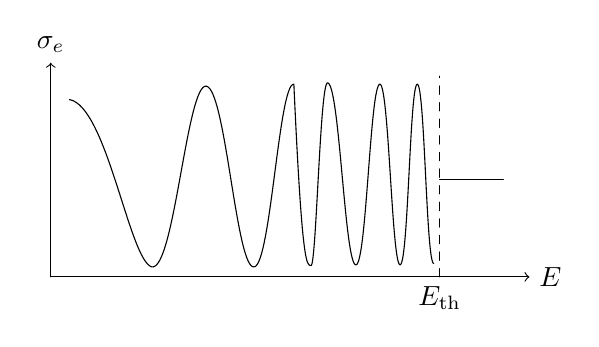
\begin{tikzpicture}[x=0.95cm,y=0.85cm,line cap=round,line join=round]
 \draw[->] (0,0) -- (6.4,0) node[right] {$E$};
 \draw[->] (0,0) -- (0,3.2) node[above] {$\sigma_e$};
 \draw[dashed] (5.2,0) -- (5.2,3.0);
 \node[below] at (5.2,0) {$E_{\mathrm{th}}$};
 \draw (0.25,2.65)
  .. controls (0.75,2.55) and (1.05,0.25) .. (1.35,0.15)
  .. controls (1.65,0.08) and (1.82,2.9) .. (2.08,2.85)
  .. controls (2.34,2.8) and (2.48,0.1) .. (2.72,0.15)
  .. controls (2.94,0.18) and (3.05,2.9) .. (3.25,2.88)
  .. controls (3.36,0.17) and (3.42,0.17) .. (3.48,0.17)
  .. controls (3.55,0.17) and (3.6,2.9) .. (3.7,2.9)
  .. controls (3.86,2.9) and (3.93,0.17) .. (4.08,0.18)
  .. controls (4.22,0.18) and (4.27,2.88) .. (4.4,2.88)
  .. controls (4.52,2.88) and (4.56,0.18) .. (4.67,0.18)
  .. controls (4.78,0.18) and (4.8,2.88) .. (4.9,2.88)
  .. controls (5.0,2.88) and (5.02,0.2) .. (5.12,0.2);
 \draw (5.2,1.45) -- (6.05,1.45);
\end{tikzpicture}
\caption{}
\end{figure}
